\subsection{28 августа. Д.р. Чиринкол}

\textit{Метеоусловия: утром, днём, вечером переменная облачность, кратковременные дожди}

\begin{figure}[h!]
	\centering
	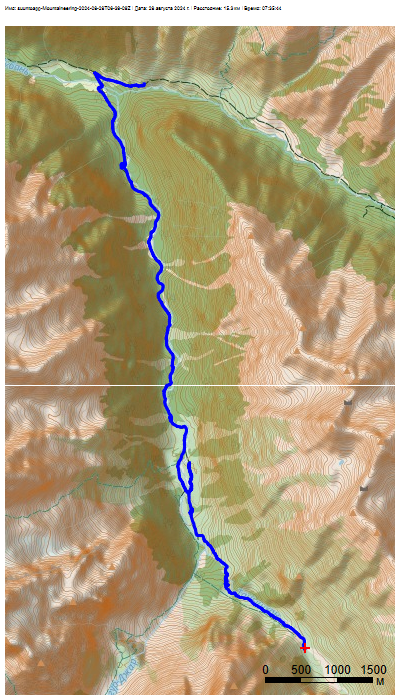
\includegraphics[angle=0, width=0.7\linewidth]{../pics/mini_maps/28}
	\label{fig:mini_28}
\end{figure}

Утром проснулись в 7:30 хорошо отдохнувшие и готовые к новому дню.

\begin{figure}[h!]
	\centering
	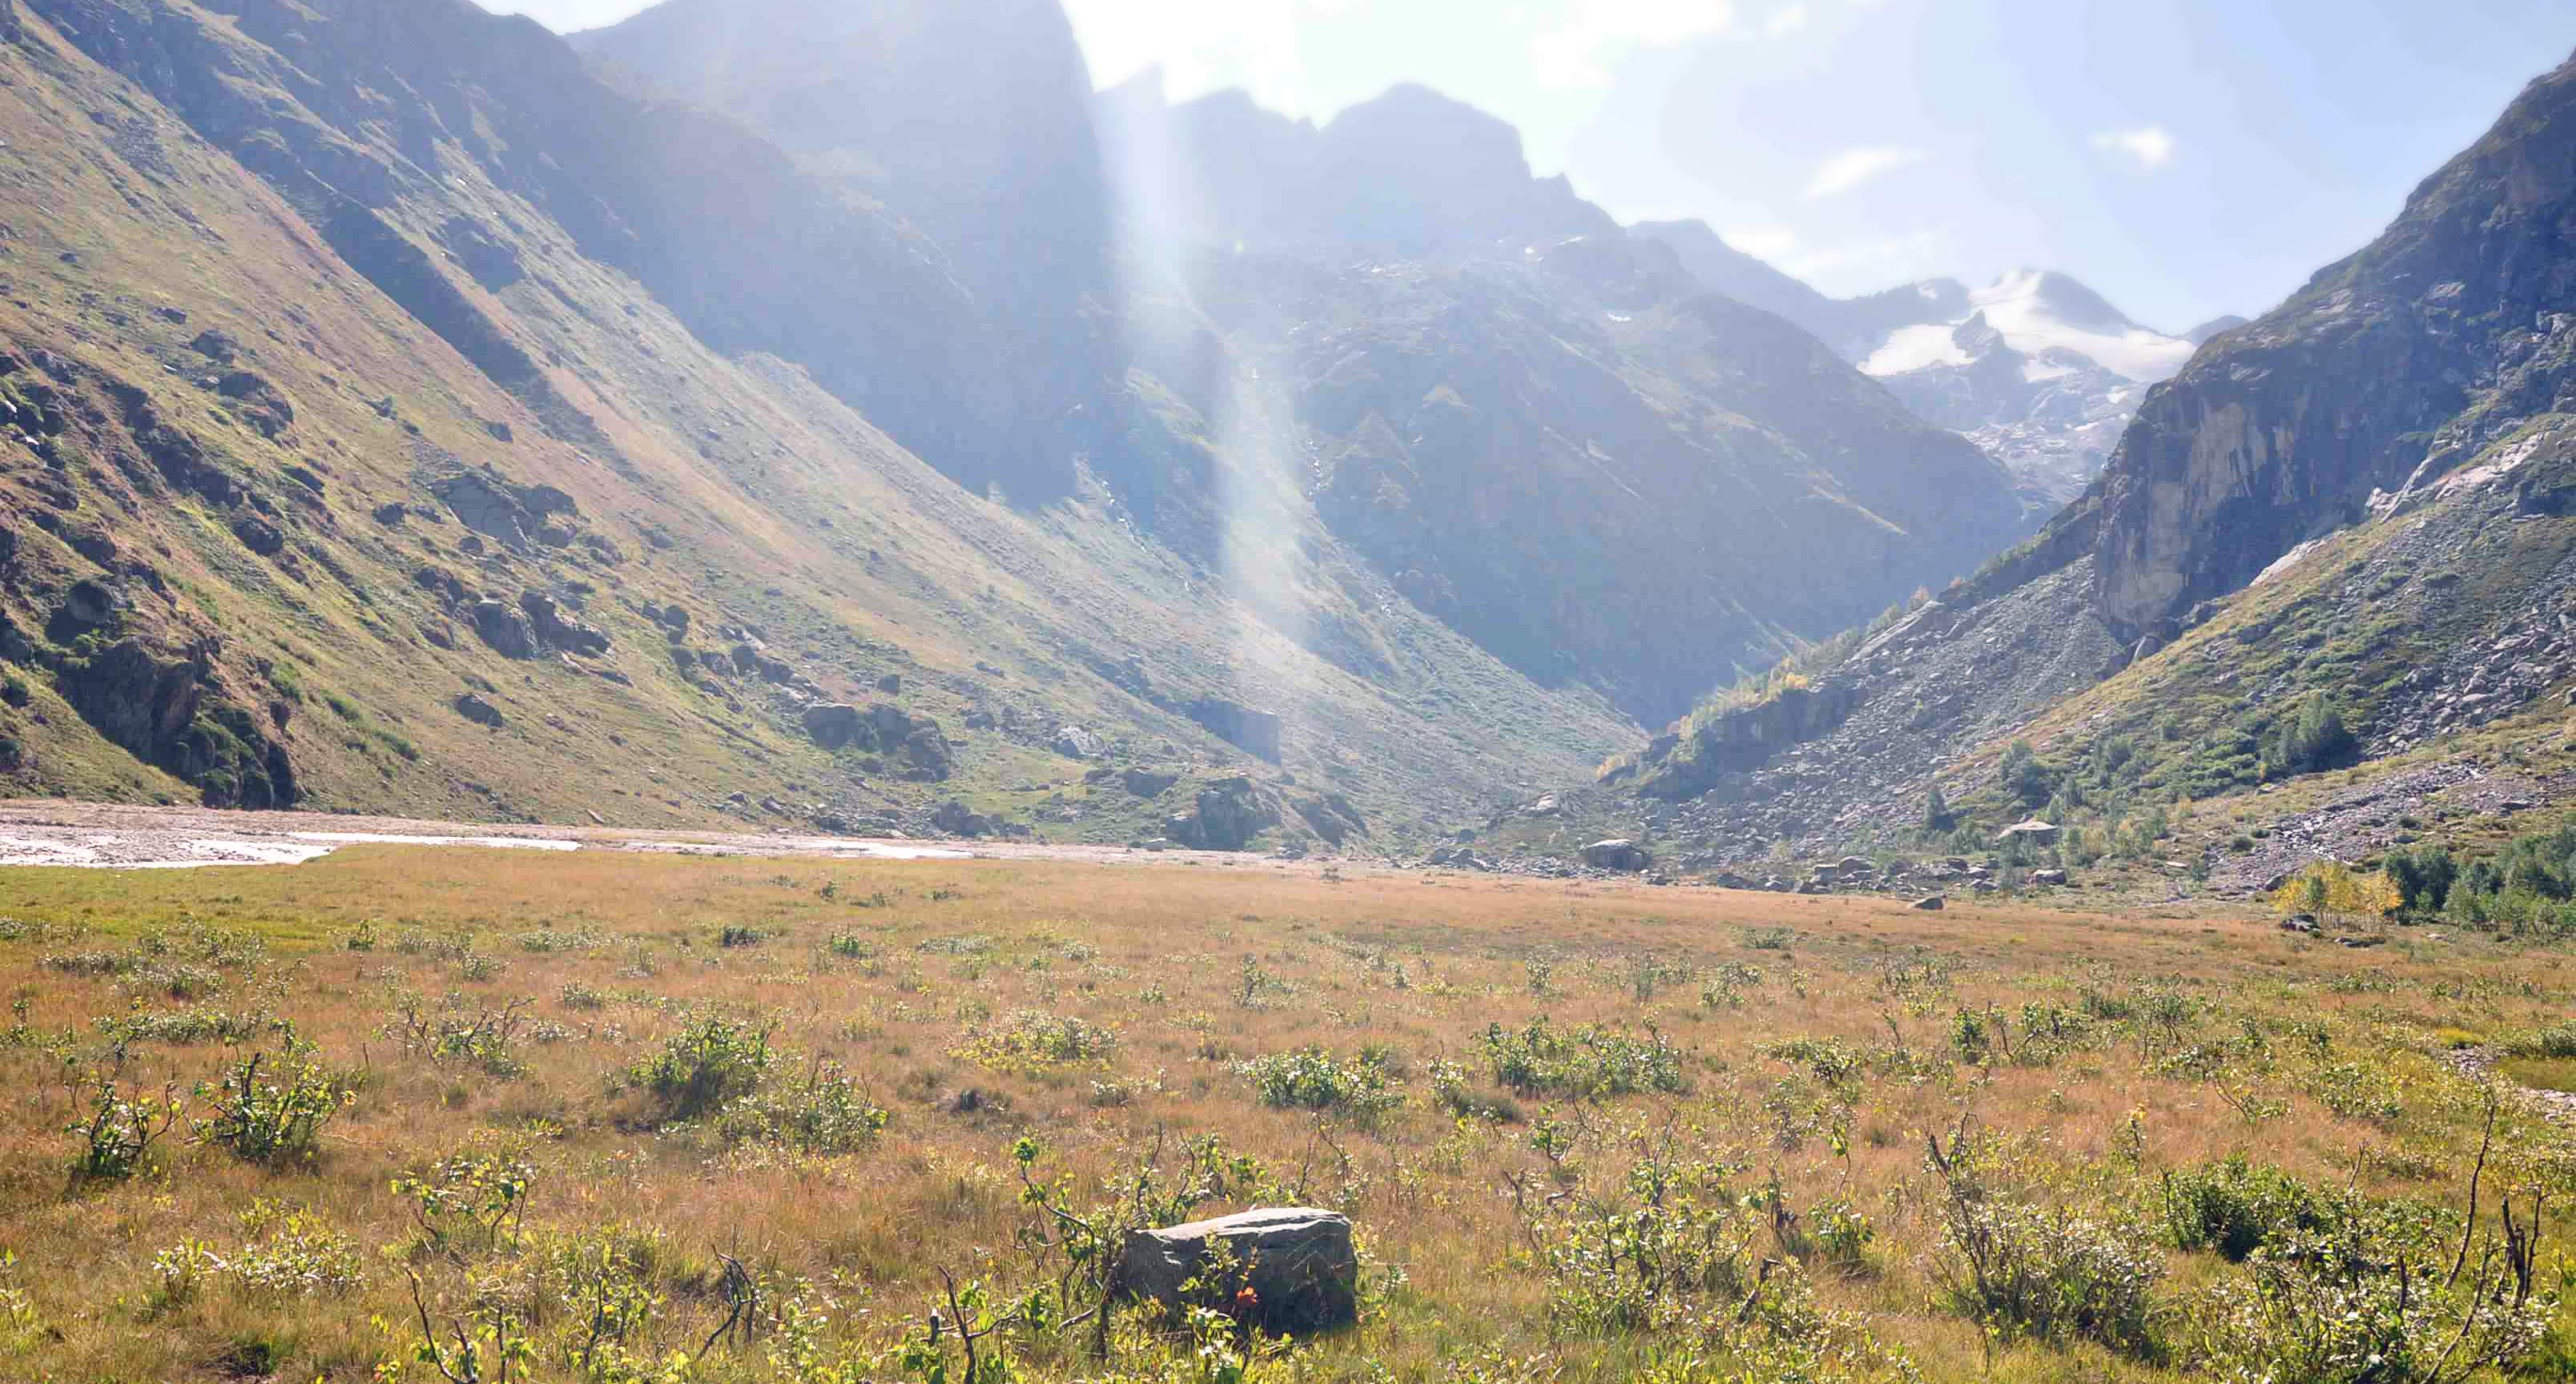
\includegraphics[width=0.7\linewidth]{../pics/DSC_0434 2.jpg}
	\caption{<<Танышханский аэродром>>~--- разлив реки. Наше м.н.}
	\label{fig:DSC_0434}
\end{figure}

 В 9:45 выдвинулись вдоль левого берега реки Танышхан вниз по течению. Тропинка пролегала через россыпи курумника, заросли берез, вечнозелёных деревьев  и рододендронов~--- идущая впереди часть группы легко терялась из виду. Здесь мы начали встречать туристов, идущих по правому берегу Танышхана налегке за ягодами. За 400 м до слияния с р. Чунгур-Джар прошли мимо добротного новопостроенного деревянного домика с небольшим хозяйством. К домику с внешним миром соединяет автомобильная грунтовка, идущая по правому берегу Танышхана. К ней от домика перекинут хороший металлический автомобильный мост, по которому мы и переходим на противоположный берег. Координаты моста: N 43.27056\degree, E 42.26168\degree. 
 
\begin{figure}[h!]
	\centering
	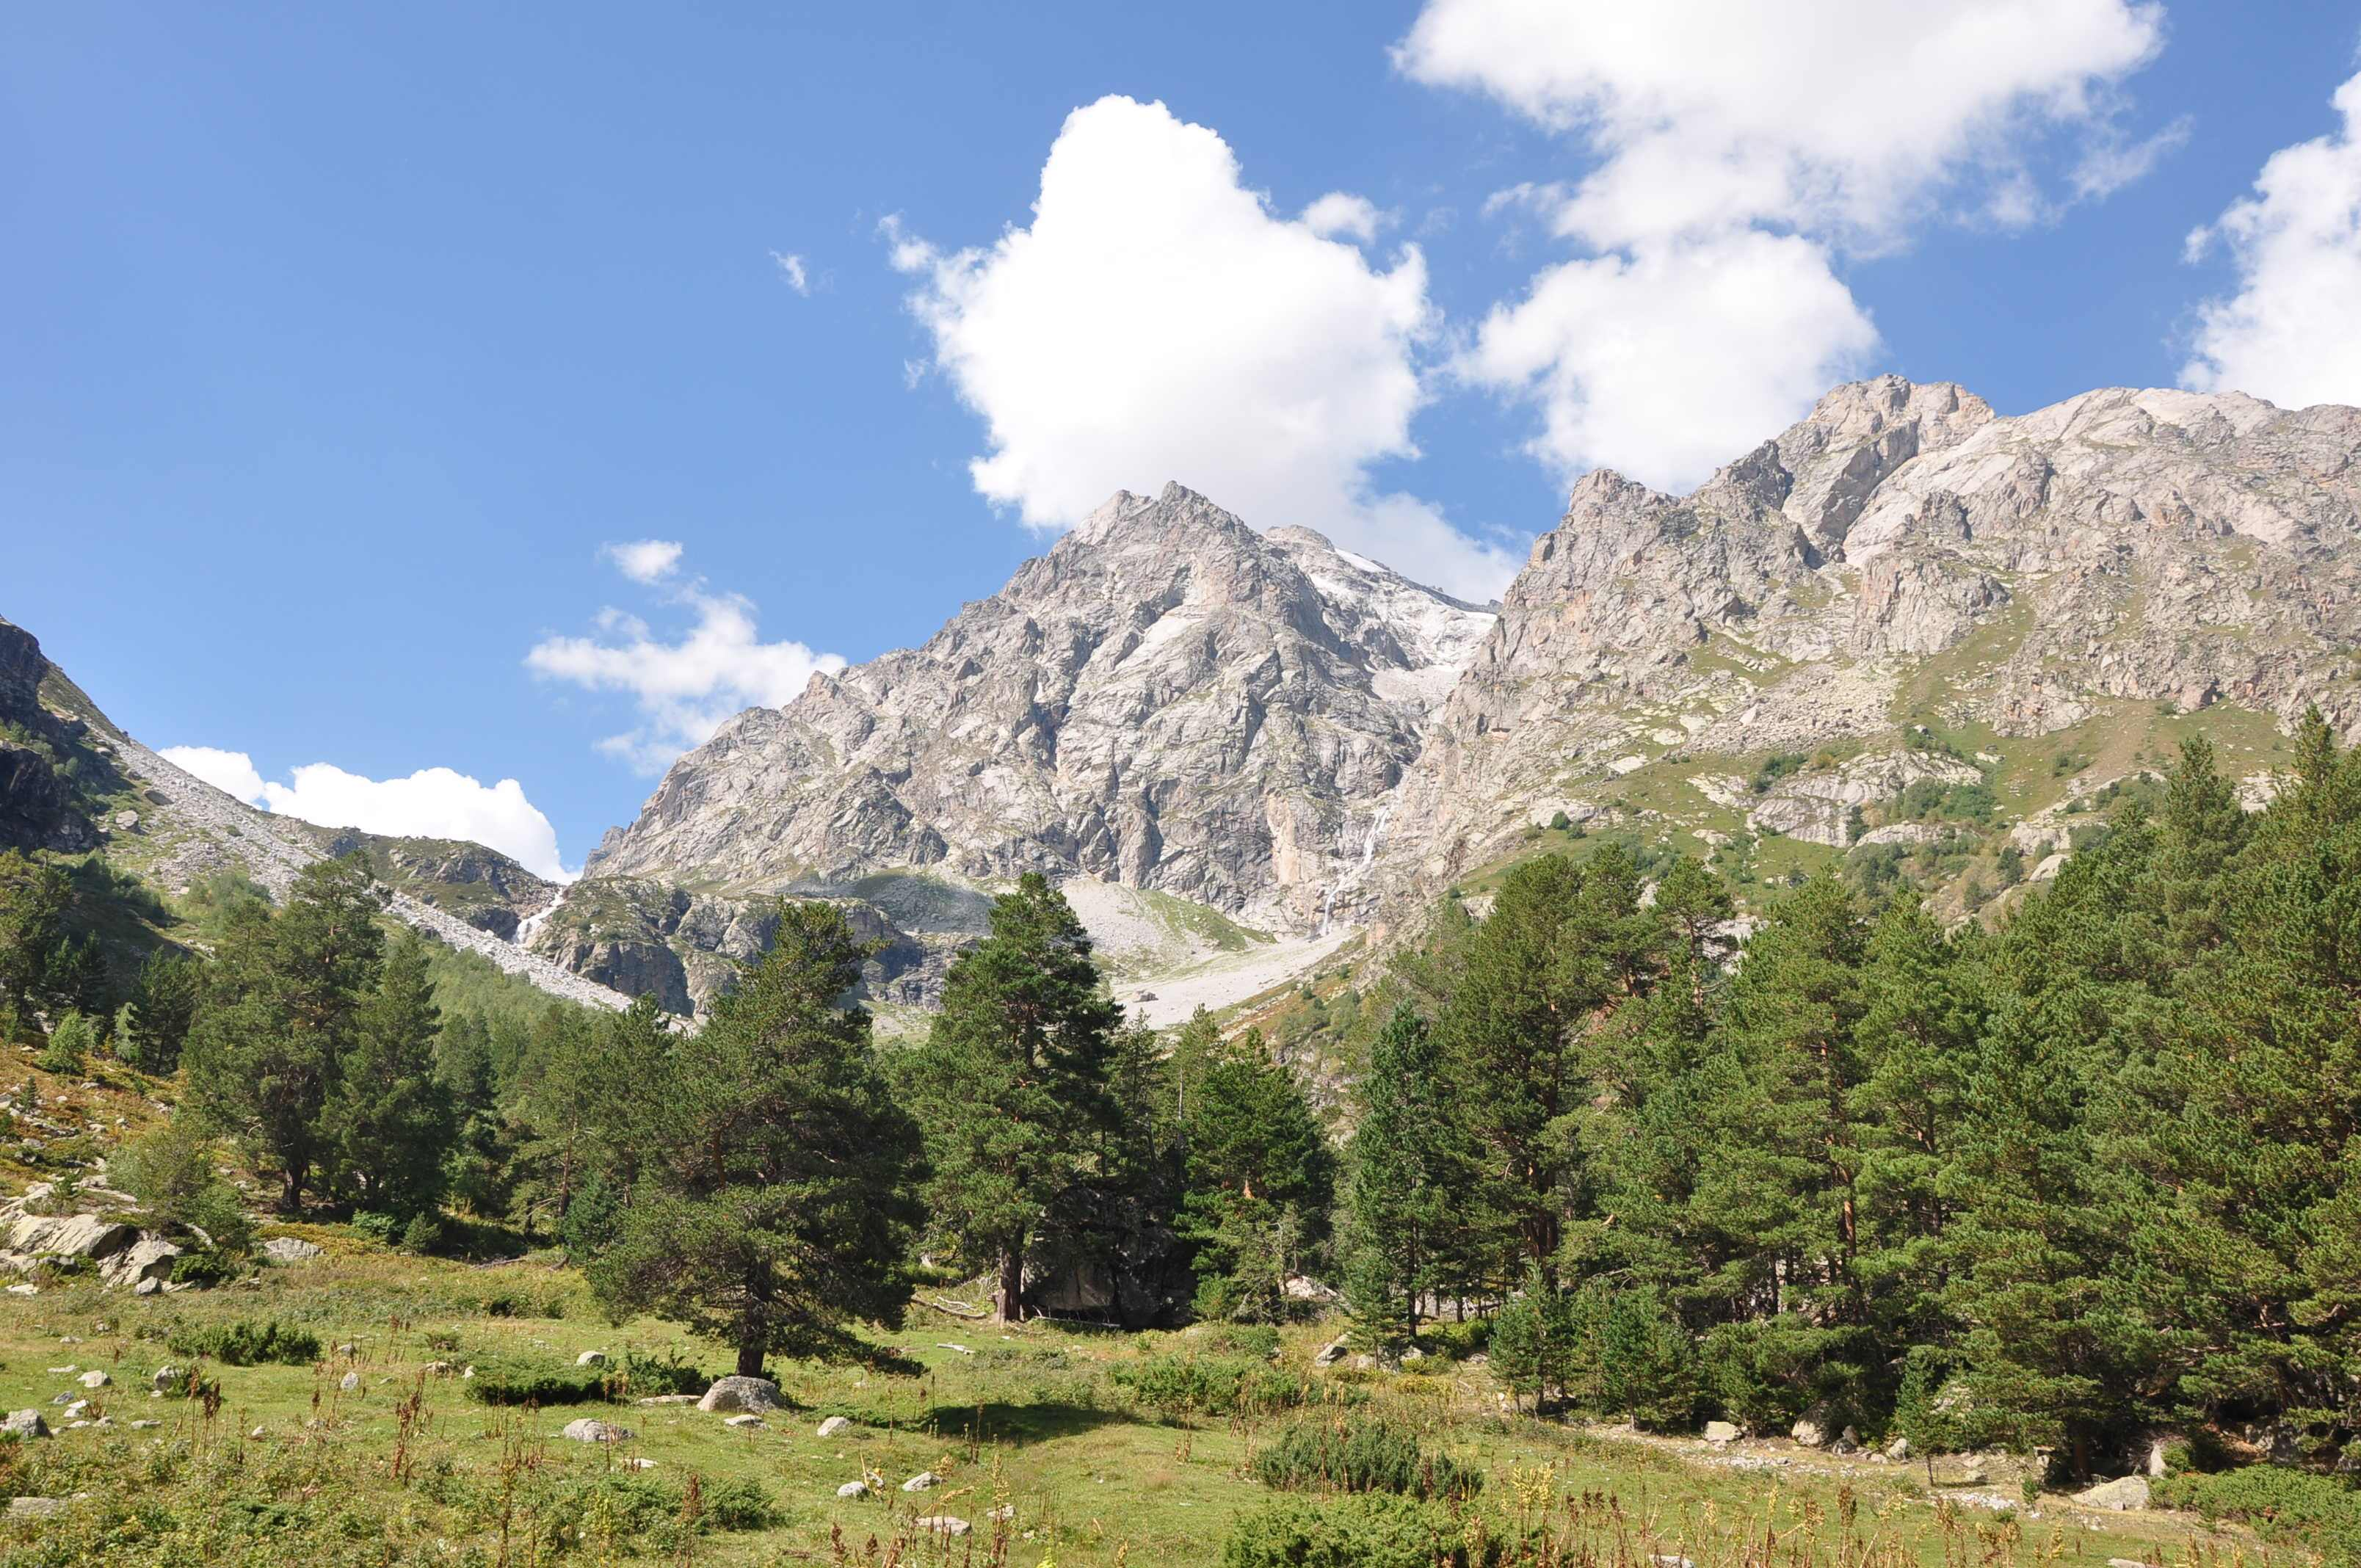
\includegraphics[width=0.7\linewidth]{../pics/DSC_0459 2}
	\caption{Д.р. Чунгур-Джар. Именно эти ступени мы обходили через пер. Перемётный}
	\label{fig:DSC_0459}
\end{figure}

Река, образующаяся от слияния Танышхана и Чунгур-Джара, называется Чиринкол (чирин - что это? Къол - это ущелье). На правом берегу в 11:10 подошли к летовкам пастухов. Повстречали как людей, так и непослушное стадо коров. Хозяйка предложила нам хычины. В 11:25 подошли к автомобильному броду, но нам не повезло и уровень воды был слишком высок, чтобы не замочить ботинки. Поэтому мы вернулись назад к коровнику и перешли по бревенчатому мосту (N 43.2798\degree,~E 42.25481\degree).

\begin{figure}[h!]
	\centering
	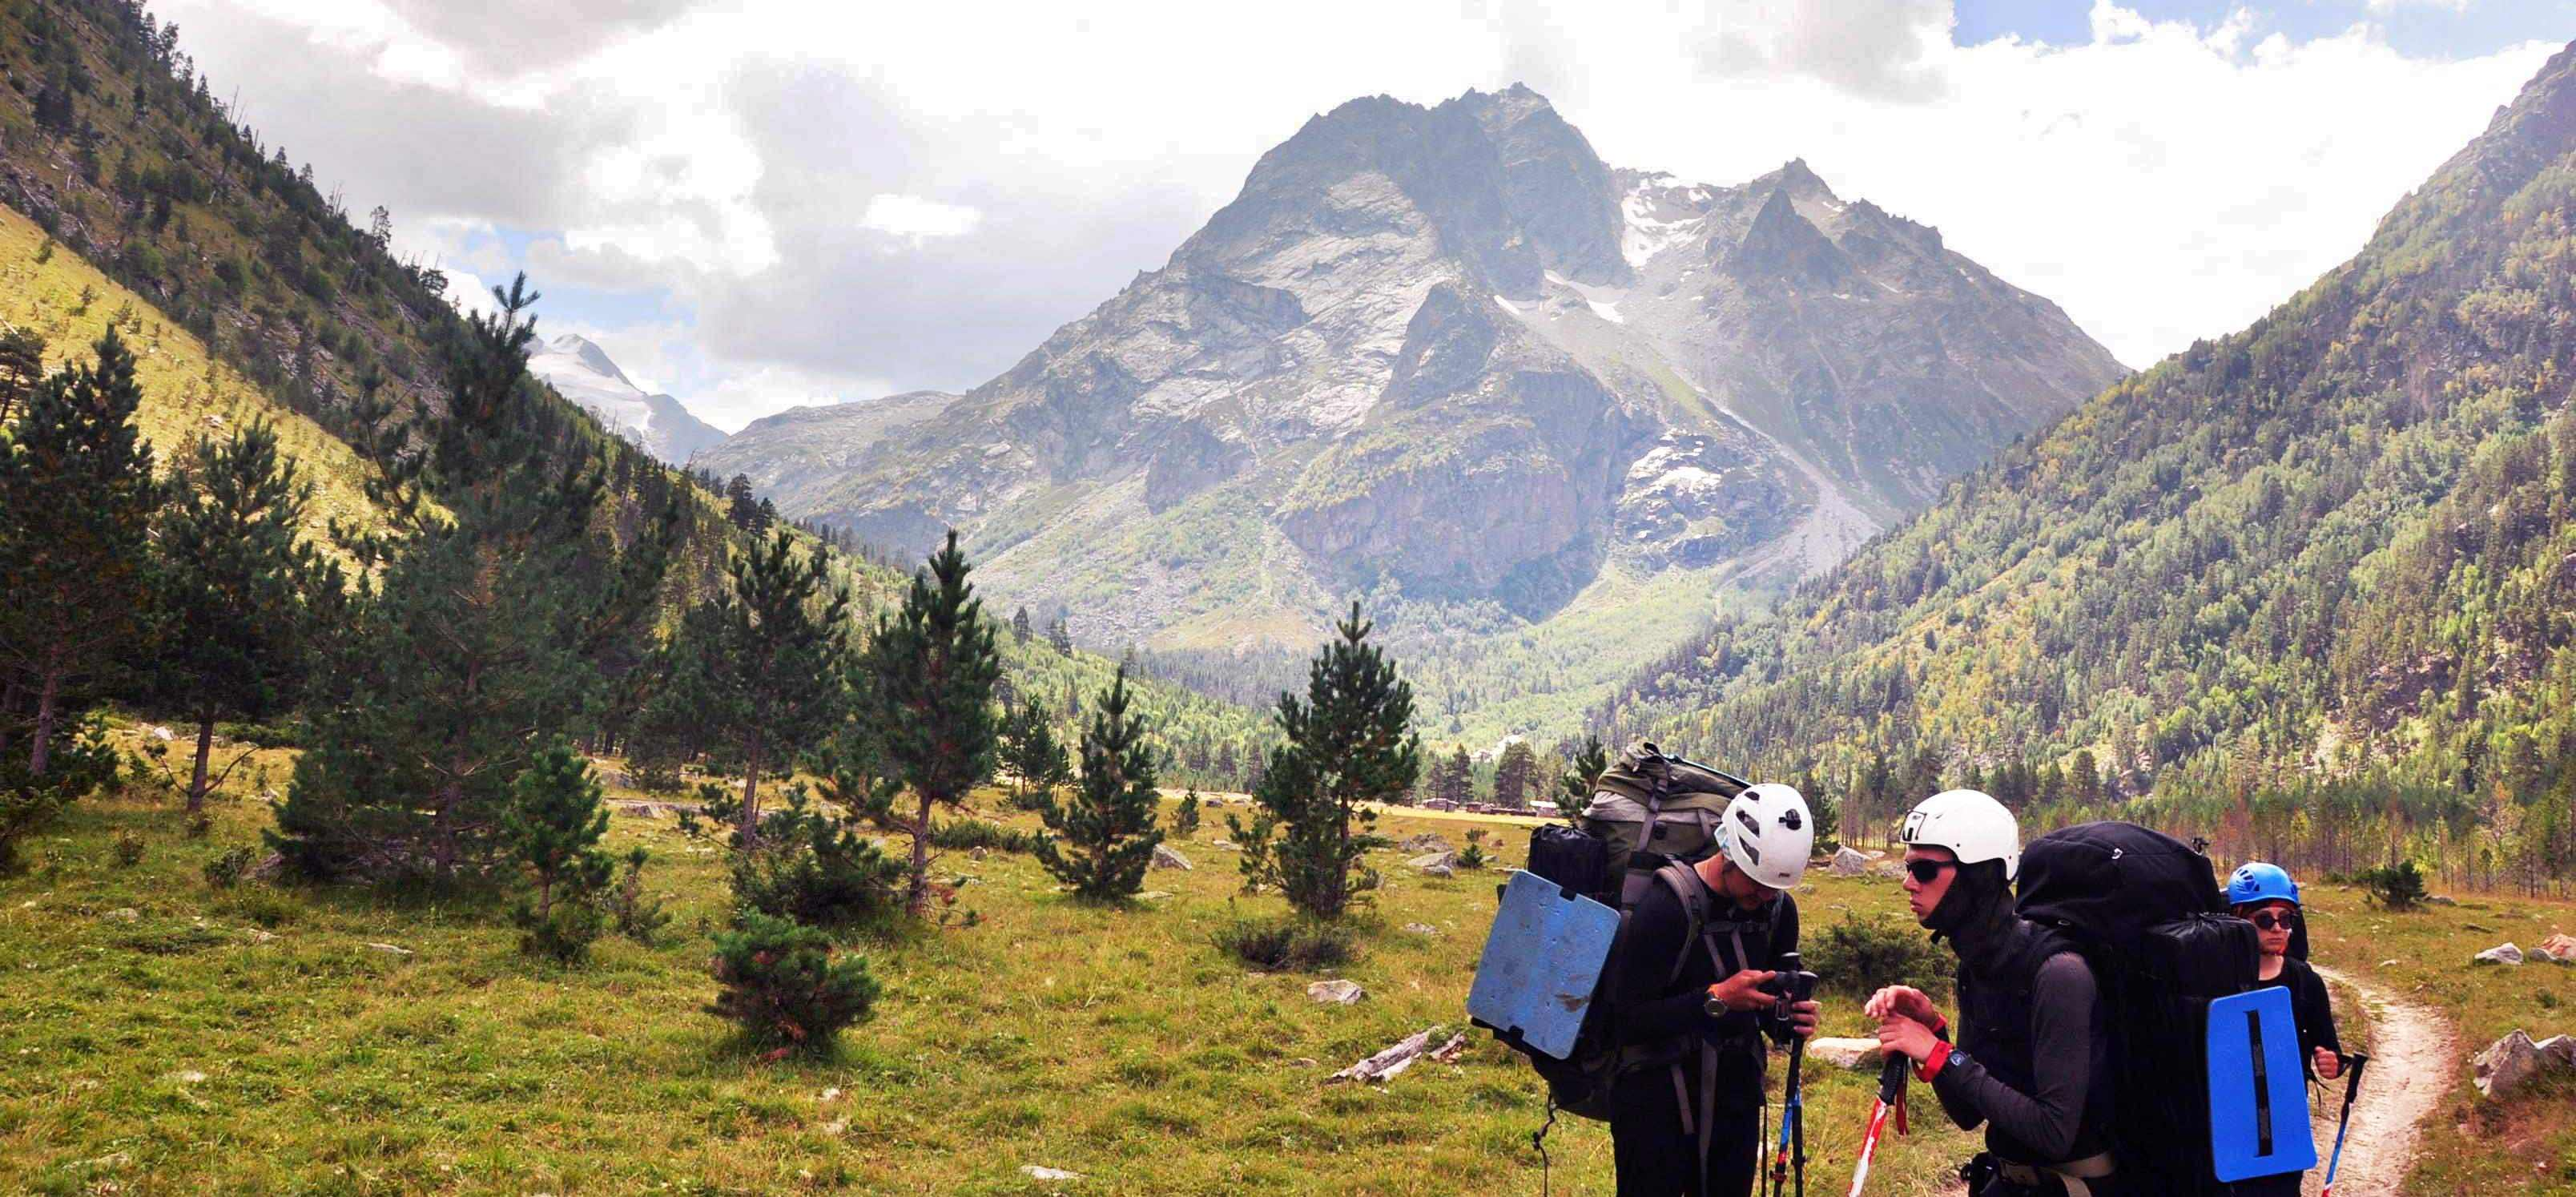
\includegraphics[width=0.7\linewidth]{../pics/DSC_0462 2}
	\caption{Д.р. Танышхан, вид на слияние р. Танышхан и Чунгур-Джар. Рядом с бродом. На заднем плане виднеется коровник}
	\label{fig:DSC_0462}
\end{figure}

Далее шли по левому берегу р. Чиринкол по проезжей дороге. 
\begin{figure}[h!]
	\centering
	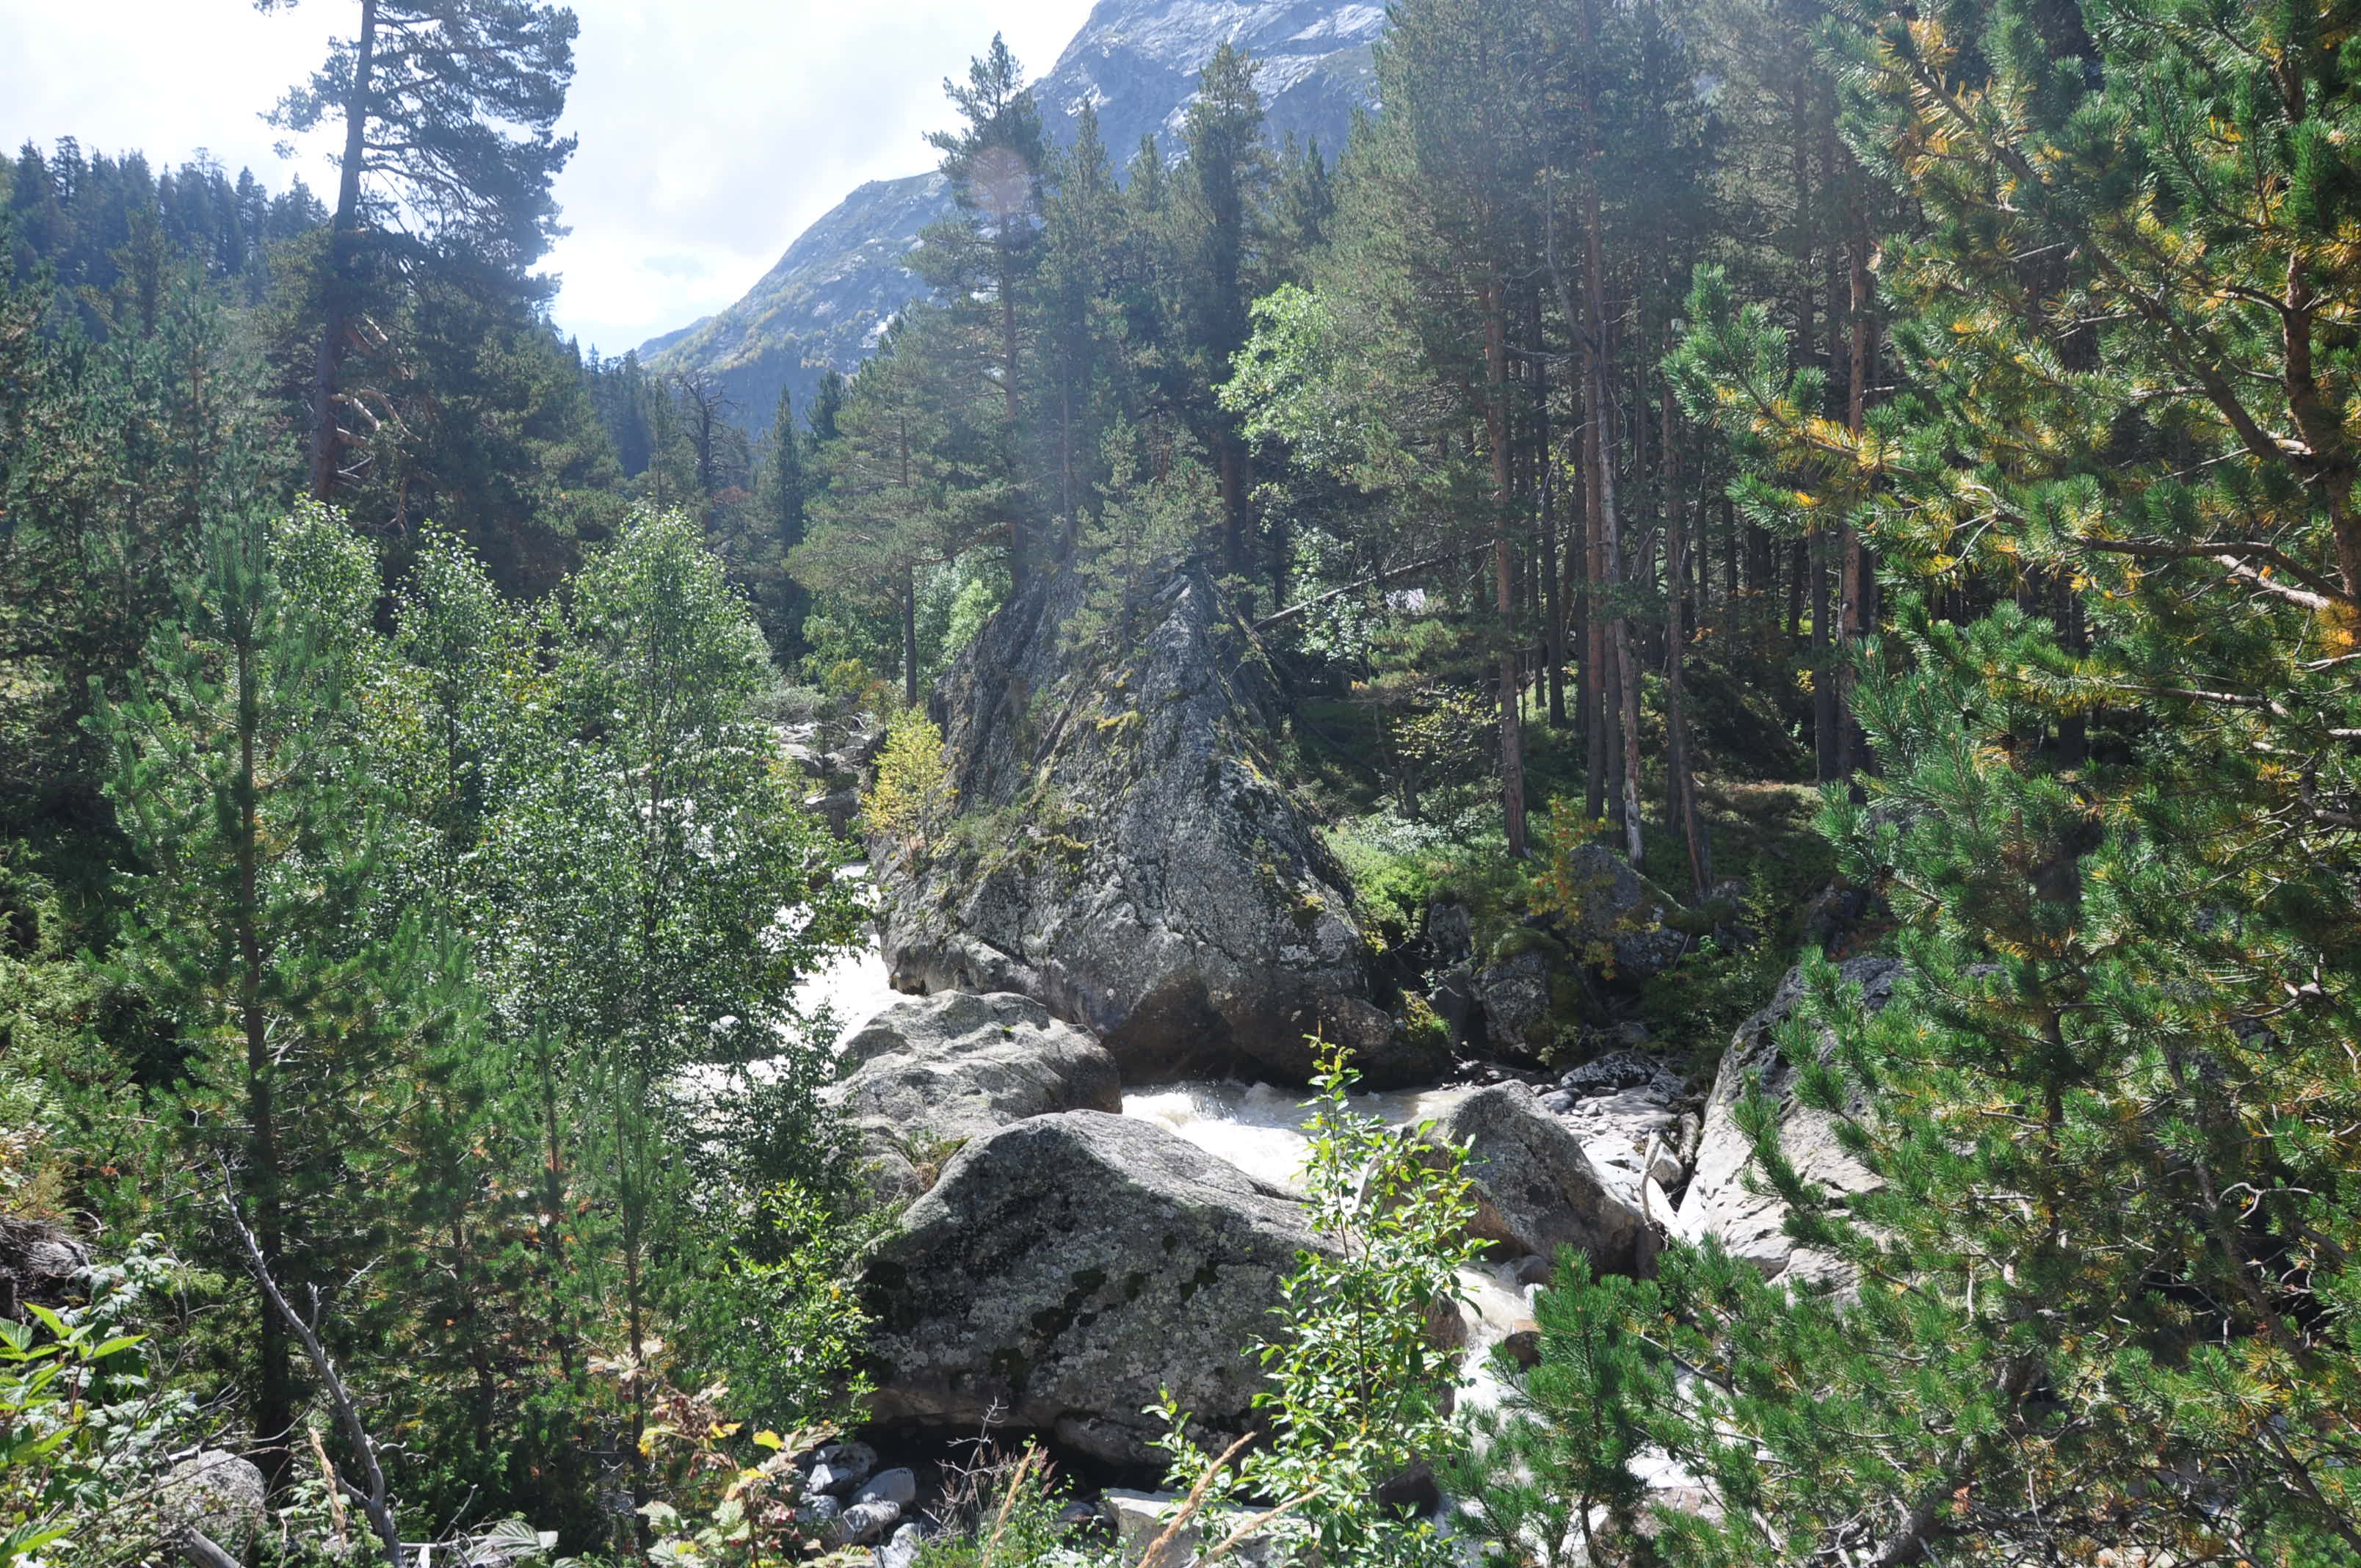
\includegraphics[width=0.7\linewidth]{../pics/DSC_0461 2}
	\caption{р. Чиринкол. Не хотелось бы в нее упасть!}
	\label{fig:DSC_0461}
\end{figure}
Пообедали в 14:14 на удобной полянке (N 43.32065° E 42.24355°). Бодро дошли до поворота на д.р. Кубань и в 17:15 встали лагерем на живописном холме (N 43.33085° E 42.24742°). Попытались поймать сеть выше по склону, но не поймали.

\clearpage